\documentclass[10pt, twocolumn]{article}
\usepackage{amsmath}
\usepackage{amsfonts}
\usepackage[margin=0.25in]{geometry}
\usepackage{pdfpages}

\newcommand*{\Perm}[2]{{}^{#1}\!P_{#2}}%
\newcommand*{\Comb}[2]{{}^{#1}C_{#2}}%
\newcommand\given[1][]{\:#1\vert\:}

\begin{document}

\section{STAT 400, Aryn Harmon}

\subsection{Midterm 1 Material}

\textbf{Probability} is a real-valued function:
1. $\mathbb{P}(S) = 1$; 2. $\mathbb{P}(A) \geq 0$; 3. If $A_1, A_2$ are mutually exclusive events, $\mathbb{P}(A_1 \cup A_2) = \mathbb{P}(A_1) + \mathbb{P}(A_2)$ and so on.\\
\textbf{Inclusion-Exclusion:} $\mathbb{P}(A \cup B) = \mathbb{P}(A) + \mathbb{P}(B) - \mathbb{P}(A \cap B)$.\\
\textbf{Conditional Probability:} $\mathbb{P}(A|B) = \frac{\mathbb{P}(A \cap B)}{\mathbb{P}(B)}$ given $\mathbb{P}(B) > 0$. $\mathbb{P}(A|B) \neq \mathbb{P}(A)$ unless $A$ and $B$ are independent. Also see Bayes's Theorem. Probability of a string of unions given $B$ is equal to the sum of the individual conditional probabilities.\\
\textbf{Multiplication Rule:} Probability of two events both occurring: $\mathbb{P}(A \cap B) = \mathbb{P}(A) \cdot \mathbb{P}(B|A)$ or $\mathbb{P}(A \cap B) = \mathbb{P}(B) \cdot \mathbb{P}(A|B)$ (one is easier than the other).\\
\textbf{Bayes's Rule:} $\mathbb{P}(A|B) = \frac{\mathbb{P}(A) \cdot \mathbb{P}(B|A)}{\mathbb{P}(B)}$. $\mathbb{P}(A)$ is the \textit{prior probability} of $A$. $\mathbb{P}(A|B)$ is the \textit{posterior probability} of $A$ given that $B$ occurred. Use to invert probabilities.\\
\textbf{Bayes's Rule 2:} $\mathbb{P}(A|B) = \frac{\mathbb{P}(A) \cdot \mathbb{P}(B|A)}{\mathbb{P}(A) \cdot \mathbb{P}(B|A) + \mathbb{P}(A') \cdot \mathbb{P}(B|A')}$.\\
\textbf{Bayes's Rule Full:} Given some partition of $S$: $A_1 \cup \dots \cup A_k = S$. $\mathbb{P}(A_i|B) = \frac{\mathbb{P}(A_i) \cdot \mathbb{P}(B|A_i)}{\sum_{m=1}^{k} \mathbb{P}(A_m) \cdot \mathbb{P}(B|A_m)}$.\\
\textbf{Independence:} $\mathbb{P}(A|B) = \mathbb{P}(A)$, $\mathbb{P}(B|A) = \mathbb{P}(B)$, and $\mathbb{P}(A \cap B) = \mathbb{P}(A) \cdot \mathbb{P}(B)$.\\
\textbf{Pairwise Independence:} All of the following must hold: $\mathbb{P}(A \cap B) = \mathbb{P}(A) \cdot \mathbb{P}(B)$, $\mathbb{P}(A \cap C) = \mathbb{P}(A) \cdot \mathbb{P}(C)$, and $\mathbb{P}(B \cap C) = \mathbb{P}(B) \cdot \mathbb{P}(C)$.\\
\textbf{Mutual Independence:} $A$, $B$, and $C$ must be pairwise independent and in addition: $\mathbb{P}(A \cap B \cap C) = \mathbb{P}(A) \cdot \mathbb{P}(B) \cdot \mathbb{P}(C)$.
\textbf{Number of ways to take $r$ objects from $n$ candidates:}

\begin{tabular}{lll}
        & Ordered Sample & Unordered Sample      \\
W. R.   & $n^r$          & ${n+r-1 \choose r}$ \\
W/o. R. & $\Perm{n}{r}$  & ${n \choose r}$   
\end{tabular}

$\Perm{n}{k}=\frac{n!}{(n-k)!}$ - permutation\\
$\binom nk=\Comb{n}{k}=\frac{n!}{k!(n-k)!}$ - combination

\textbf{Binomial Theorem:} $(a+b)^n = \sum_{r=0}^n {n \choose r} a^r b^{n-r}$. ${n \choose n-r} = {n \choose r}$, ${n \choose 0} = {n \choose n} = 1$, ${n \choose 1} = {n \choose n-1} = n$.\\
\textit{Some magic formulae:} 1. $\sum_{r=0}^n {n \choose r} = 2^n$. 2. $\sum_{r=0}^n (-1)^r {n \choose r} = 0$. 3. $\sum_{r=0}^n {n \choose r} p^r (1-p)^{n-r} = 1$.\\
\textbf{Pascal's Equation:} ${n \choose r} = {n-1 \choose r} + {n-1 \choose r-1}$.\\
\textbf{Hypergeometric Distribution:} $f(x) = \mathbb{P}(X=x) = \frac{{N_1 \choose x} \cdot {N_2 \choose n-x}}{{N \choose n}}$, where $x \leq n$, $x \leq N_1$, $n-x \leq N_2$ and $N = N_1 + N_2$. $\mathbb{E}(X) = n\frac{N_1}{N}$ and $Var(X) = n \cdot \frac{N_1}{N} \cdot \frac{N_2}{N} \cdot \frac{N-n}{N-1}$. Example: Urn model: $N_1$ red balls, $N_2$ blue balls, draw $n$ balls from $N_1 + N_2$ balls, then look at the probability that there are $x$ red balls in the selected $n$ balls.\\
\textbf{Mean:} $\mu = \mathbb{E}(X) = \sum_{x \in S} x f(x)$.\\
\textbf{Variance:} $\sigma^2 = Var(X) = \mathbb{E}(X - \mu)^2 = \mathbb{E}(X^2) - \mu^2 = \sum_{i=1}^{k} x_i^2 f(x_i) - \mu^2$. \textbf{Standard Deviation:} $\sigma$.\\
\textbf{r-th Moment:} $\mathbb{E}(|X|^r) = \sum_{x \in S} |x|^r f(x) < \infty$; is the moment about the origin.\\
\textbf{r-th Moment about $b$:} $\mathbb{E}((X-b)^r) = \sum_{x \in S} (x-b)^r f(x)$; is the moment about $b$. Facts: $\mu$ is the first moment of $X$ about the origin. $\sigma^2$ is the second moment of $X$ about $\mu$.\\
\textit{Example of Variance Properties:} $Var(aX+b) = a^2 \cdot Var(X)$.
\textbf{Bernoulli Distribution:} A random experiment is called a set of Bernoulli trials if each trial has only two outcomes, has a constant $p$, and each trial is independent. $f(x) = p$ if $x=1$, $1-p$ if $x=0$, with $0 \leq p \leq 1$. $\mathbb{E}(X) = p$ and $Var(X) = p(1-p)$.\\
\textbf{Binomial Distribution:} Let $X$ be the number of successes in $n$ independent Bernoulli trials with $p$. Then $X \sim b(n,p)$. $f(x) = \mathbb{P}(X=x) = {n \choose x} p^x (1-p)^{n-x}$. $\mathbb{E}(X) = np$ and $Var(X) = np(1-p)$.\\
A note: binomial and hypergeometric are similar, but binomial has replacement and one category, and hypergeometric has two categories and no replacement.\\
\textbf{Cumulative Distribution Function:} $F(x) = \mathbb{P}(X \leq x), x \in (-\infty, \infty)$. For discrete random variables: $f(x) = \mathbb{P}(X=x) = \mathbb{P}(X \leq x) - \mathbb{P}(X \leq x - 1) = F(x) - F(x-1)$.\\
\textbf{Geometric Distribution:} $f(x) = p(1-p)^{x-1}, x = 1,2,3,\dots$. $X$ represents the draw in which the first success is drawn. $f(x)$ is the probability of getting a success in the $x$-th draw.\\
\textbf{Negative Binomial Distribution:} $f(x) = {x-1 \choose r-1} p^r (1-p)^{x-r}$ and $x = r,r+1,r+2,\dots$. $X$ is the number of trials it takes to get $r$ successes. $f(x)$ is the probability that the $r$-th success occurs on the $x$-th trial.

\subsection{Midterm 2 Material}
\textbf{Moment Generating Function:} $M(t) = \mathbb{E}(e^{tX}) = \sum_{x \in S}{e^{tX}f(x)}$ if $f(x)$ is the p.d.f. of some distribution and $t \in V_h(0)$ is finite. \textit{Theorem:} $\mathbb{E}(X^r) = M^{(r)}(0)$, so $\mu = \mathbb{E}(X) = M'(0)$ and $\sigma^2 = \mathbb{E}(X^2) - [\mathbb{E}(X)]^2 = M''(0) - [M'(0)]^2$. To calculate the m.g.f. and p.d.f. of some random variable given only its moments, use the Taylor series expansion centered at zero. $M(t) = M(0) + M'(0)\left(\frac{t}{1!}\right) + M''(0)\left(\frac{t^2}{2!}\right) + \dots = 1 + \mathbb{E}(X)\left(\frac{t}{1!}\right) + \mathbb{E}(X^2)\left(\frac{t^2}{2!}\right) + \dots$.\\
\textbf{Poisson distribution:} \textit{Definition:} Poisson process counts the number of events occurring in a fixed time/space given a rate $\lambda$. Let $X_t$ be the number events which occur in $t$ unit time intervals. $\mathbb{P}(X_t = x) = \frac{(\lambda t)^x}{x!} e^{-\lambda t}$. $\mu = \lambda, \sigma^2 = \lambda$.\\
\textbf{Poisson Approximation} of Binomial Distribution: If $X \sim b(n,p)$ and $n$ is large while $p$ is small, then $X$ can be approximated as $\hat{X} \sim poi(\lambda) \, s.t. \, \lambda = np$.\\
\textbf{Mean:} $\mu = \int_{-\infty}^{\infty} x f(x) dx$.\\
\textbf{Variance:} $\sigma^2 = \int_{-\infty}^{\infty} (x - \mu)^2 f(x) dx$.\\
\textbf{M.G.F.:} $M(t) = \mathbb{E}(e^{tX}) = \int_{-\infty}^{\infty} e^{tx} f(x) dx, t \in (-h,h)$.\\
\textbf{Percentile:} $p = \int_{-\infty}^{\pi_p} f(x) dx = F(\pi_p)$.\\
\textbf{Uniform Distribution:} $f(x) = \frac{1}{b-a}, a \leq x \leq b$. If $X \sim U(a,b)$, then $\mathbb{E}(X) = \frac{a+b}{2}$, $\sigma^2 = \frac{(b-a)^2}{12}$, and $M(t) = \mathbb{E}(e^{tX}) = \frac{e^{tb} - e^{ta}}{t(b-a)}, t \neq 0$ and $M(0) = 1$.\\
\textbf{Exponential Distribution:} This describes the waiting time between events in a Poisson process with rate $\lambda$. Let $\theta = \frac{1}{\lambda}$. Then if $X \sim Exp(\theta)$, $f(x) = \frac{1}{\theta}e^{-\frac{x}{\theta}}, x \geq 0$ and 0 otherwise. $\mu = \theta$, $\sigma^2 = \theta^2$, and $M(t) = (1 - \theta t)^{-1}, t < \frac{1}{\theta}$.\\
\textbf{Memoryless Property} of the Exponential Distribution: What happened in the past does not matter now. Only the present can determine the future. $\mathbb{P}(X > a+b \given[\big] X > a) = \mathbb{P}(X > b), \forall a, b \geq 0$.\\
\textbf{Gamma Function:} $\Gamma(x) = \int_{0}^{\infty} y^{x-1} e^{-y} dy, \, x > 0$.\\
\textbf{Gamma Distribution:} $f(t)$ represents the waiting time unitl the $\alpha$-th occurrence of some Poisson process with rate $\lambda$. $f(t) = \frac{\lambda^\alpha t^{\alpha-1}}{(\alpha-1)!} e^{-\lambda t}, \, t \geq 0$. Then let $\theta = \lambda^{-1}$, then $f(t) = \frac{1}{\Gamma(\alpha)} \theta^{\alpha} t^{\alpha - 1} e^{\frac{-t}{\theta}}, \, t \geq 0, \, \alpha \in \mathbb{R}$. $\mu = \alpha \theta$, $\sigma^2 = \alpha \theta^2$, and $M(t) = (1 - \theta t)^{-\alpha}$. If $\alpha = 1$, $\mathrm{gamma}(1,\theta) = \mathrm{Exp}(\theta)$.\\
\textbf{$\chi^2$ Distribution:} If $X \sim \mathrm{gamma}(\alpha,\theta)$, and $\theta = 2$ and $\alpha = \frac{r}{2}$, where $r$ is a positive integer, then $X$ is a $\chi^2$ distribution with degree of freedom $r$. $X \sim \chi^2(r)$. $\mu = r$, $\sigma^2 = 2r$, and $M(t) = (1-2t)^{\frac{-r}{2}}, \, t < \frac{1}{2}$. $e^2 = \chi^2(2)$.\\
\textbf{Normal Distribution:} Bell curve! $f(x) = \frac{1}{\sqrt{2\pi}\sigma} e^{-\frac{(x-\mu)^2}{2\sigma^2}}, \, x \in \mathbb{R}$. $X \sim N(\mu, \sigma^2)$. $X \sim N(0, 1)$ is the standard normal distribution. $\mu = \mu$, $\sigma^2 = \sigma^2$, and $M(t) = e^{\mu t + \frac{\sigma^2 t^2}{2}}$. Standardization: $X \sim N(\mu, \sigma^2)$, then $Z = \frac{X-\mu}{\sigma} \sim N(0, 1)$.\\
\textbf{Normal Square Distribution:} Let $X \sim N(\mu, \sigma^2)$ and $Z = \frac{X-\mu}{\sigma}$. Then the random variable $V = Z^2 \sim \chi^2(1)$.\\
\textbf{Cauchy Distribution:} (Why do we even need this distribution?) $f(x) = \frac{1}{\pi (1 + x^2)}, \, x \in \mathbb{R}$. Symmetric about zero, so median is zero, but $\mu$ is undefined because the tail of the p.d.f. is too heavy (i.e. each integral of the distribution does not converge). $c.d.f. = F(x) = \frac{1}{\pi} \arctan(x) + \frac{1}{2}, \, x \in \mathbb{R}$.\\
\textbf{Joint Probability Density Function:} $\mathbb{P}((X, Y) \in A) = \int\int f(x,y) dx dy$.\\
\textbf{Marginal Probability Density Function:} $f_x(x) = \int_{-\infty}^{\infty} f(x,y) dy$ and the other way around for $y$.\\
\textbf{Mathematical Expectation:} $\mathbb{E}[g(X,Y)] = \int_{-\infty}^{\infty} \int_{-\infty}^{\infty} g(x,y) f(x,y) dx dy$.\\
\textbf{Independent Random Variables:} Two events $A$ and $B$ are independent iff $f(x,y) = f_x(x) \cdot f_y(y) \, \forall x,y$. This works for both the p.d.f. and the c.d.f.\\
\textbf{Trinomial Distribution:} This is an extension of the binomial distribution into two dimensions. $f(x_1,x_2) = \mathbb{P}(X_1 = x_1, X_2 = x_2) = \frac{n!}{x_1! x_2! (n - x_1 - x_2)!} p_1^{x_1} p_2^{x_2} (1 - p_1 - p_2)^{n - x_1 - x_2}$ for $x_1, x_2 \geq 0$, $x_1 + x_2 \leq n$.\\
\textbf{Covariance:} $Cov(X,Y) = \mathbb{E}[(X - \mu_x)(Y - \mu_y)], \mu_x = \mathbb{E}(X), \mu_y = \mathbb{E}(Y)$. Useful identity: $Cov(X,Y) = \mathbb{E}(XY) - \mathbb{X}\mathbb{E}(Y)$.\\
\textbf{Properties of Covariance:} Zero-angle: $Cov(X,X) = Var(X)$. Symmetry: $Cov(X,Y) = Cov(Y,X)$. $Cov(aX + b, Y) = a \cdot Cov(X,Y)$. $Cov(X+Y, W) = Cov(X,W) + Cov(Y,W)$. $Cov(aX+bY, cX+dY) = (ac) \cdot Var(X)+(bd) \cdot Var(Y)+(ad+bc) \cdot Cov(X, Y)$. $Var(aX + bY) = a^2 \cdot Var(X) + 2ab \cdot Cov(X, Y) + b^2 \cdot Var(Y)$.\\
\textbf{Correlation Coefficient:} $\rho_{XY} = \frac{\sigma_{XY}}{\sigma_X \cdot \sigma_Y} = \frac{Cov(X,Y)}{\sqrt{Var(X)} \cdot \sqrt{Var(Y)}}$. Uncorrelated: $\rho_{XY} = 0 \Leftrightarrow \sigma_{XY} = 0$. If $X$ and $Y$ are independent, then $\rho_{XY} = 0$, but the implication \textbf{does not} go the other way.\\
\textbf{I.I.D.:} If every marginal probability density function is equal and independent, then all of the random variables are independent and identically distributed (i.i.d.).\\
\textbf{Combinations:} If $Y$ is a linear combination of independent random variables with constant multiples, then the expectation of $Y$ is simply the sum of the expectations of random variables. The variance of $Y$ is the sum of the variances of the random variables with their constant multiples squared. The moment of a linear combination of random variables is the product of their individual moments.\\
\textbf{Summary of Combinations:} Suppose $X$ and $Y$ are independent. Then,
\begin{itemize}
        \item $bern(p) + bern(p) = b(2,p)$
        \item $b(n_1,p) + b(n_2,p) = b(n_1 + n_2, p)$
        \item $geo(p) + geo(p) = negbin(2,p)$
        \item $negbin(r_1,p) + negbin(r_2,p) = negbin(r_1 + r_2, p)$
        \item $poi(\lambda_1) + poi(\lambda_2) = poi(\lambda_1 + \lambda_2)$
        \item $exp(\theta) + exp(\theta) = gamma(2,\theta)$
        \item $gamma(\alpha_1,\theta) + gamma(\alpha_2,\theta) = gamma(\alpha_1 + \alpha_2, \theta)$
        \item $N(\mu_1,\sigma_1^2) + N(\mu_2,\sigma_2^2) = N(\mu_1 + \mu_2,\sigma_1^2 + \sigma_2^2)$
\end{itemize}

\subsection{Final Material}
Everything taught in the class is on the final.\\
\textbf{Chebyshev's Inequality:} If $k \geq 1$: $\mathbb{P}(|X - \mu| \geq k \sigma) \leq \frac{\sigma^2}{\epsilon^2}$. Let $\epsilon = k \sigma$: $\mathbb{P}(|X - \mu| \geq \epsilon) \leq \frac{1}{k^2}$.\\
\textbf{Central Limit Theorem (CLT):} $\frac{\sqrt{n}(\overline{X} - \mu)}{\sigma} \rightarrow Z, \;\mathrm{as}\; n \rightarrow \infty$.\\
\textbf{Normal Approximation to Binomial:} If $np \geq 5$ and $n(1-p) \geq 5$, then\\
\begin{tabular}{lll}
        & $b(n,p)$ & $N(\mu,\sigma^2)$     \\
Mean    & $np$          & $\mu$ \\
Variance& $np(1-p)$  & $\sigma^2$   
\end{tabular}\\
\textbf{Normal Approximation to Poisson:}\\
\begin{tabular}{lll}
        & Poisson$(\lambda)$ & $N(\mu,\sigma^2)$     \\
Mean    & $\lambda$          & $\mu$ \\
Variance& $\lambda$  & $\sigma^2$   
\end{tabular}\\
\textbf{Jensen's Inequality:} If $g : \mathbb{R} \rightarrow \mathbb{R}$ is a convex function and $X$ is a random variable, then $\mathbb{E}[g(X)] \geq g(\mathbb{E}(X))$.\\
\textbf{Maximum Likelihood Estimator:} Maximize the likelihood function subject to the parameter space.
\begin{enumerate}
	\item Construct likelihood function, $F(x; \theta) = \Pi_{i=1}^{n}(f(x_i))$.
	\item If applicable, take the log of this to make things easier to differentiate and to change the product into a sum. $l(x; \theta)$.
	\item Differentiate to get $\frac{dl(x;\theta)}{d\theta}$.
	\item Assume convexity (ha) and find optimal $\theta$ by solving $\frac{dl(x;\theta)}{d\theta} = 0$.
\end{enumerate}
\textbf{Sample Mean:} $\frac{1}{n}\sum_{i=1}^{n}X_i \equiv \overline{X}$.\\
\textbf{Sample Variance:} For $z$ distribution: $\frac{1}{n}\sum_{i=1}^{n}(X_i - \overline{X})^2$, and for $t$ distribution: $\frac{1}{n-1}\sum_{i=1}^{n}(X_i - \overline{X})^2$.\\
\textbf{Method of Moments Estimator:} Construct a system of equations using moments and sample data. For example, equate theoretical mean with sample mean, and theoretical variance with sample variance, then solve. \texttt{<><><maybe put an example here<><>><}\\
\textbf{Helpful Distribution Values:}\\
\begin{tabular}{ll}
$\alpha$ & $z_{1-\alpha}$ \\
0.2      & 0.840 \\
0.1      & 1.280 \\
0.05     & 1.645 \\
0.025    & 1.960 \\
\end{tabular}\\
\textbf{Confidence Intervals for Means:}\\
\tiny
\begin{tabular}{rcc}
                & Known Variance & Unknown Variance     \\
Two Side       & $\left[ \overline{X} - z_{\frac{\alpha}{2}} \frac{\sigma}{\sqrt{n}}, \overline{X} + z_{\frac{\alpha}{2}} \frac{\sigma}{\sqrt{n}} \right]$ & $\left[ \overline{X} - t_{\frac{\alpha}{2}}(n-1) \frac{S}{\sqrt{n}}, \overline{X} + t_{\frac{\alpha}{2}}(n-1) \frac{S}{\sqrt{n}} \right]$ \\
Lower & $\left[ \overline{X} - z_{\alpha} \frac{\sigma}{\sqrt{n}}, \infty \right)$ & you can \\
Upper & $\left( -\infty, \overline{X} + z_{\alpha} \frac{\sigma}{\sqrt{n}} \right]$ & figure it out \\
\end{tabular}\\
\normalsize
$S^2 = \frac{1}{n-1}\sum_{i=1}^{n}(X_i - \overline{X})^2$ be the sample variance. 
When the population distribution is normal, use the ($n-1$) version unless you need to use MLE for which the ($n$) version is needed. For other distributions, use the ($n$) version. If no distribution is mentioned, then assume it to be normal and use the ($n-1$) version.\\
\textbf{Confidence Interval for Variance:} $\left[ \frac{(n-1)S^2}{b}, \frac{(n-1)S^2}{a} \right], a=\chi_{1-\frac{\alpha}{2}}^2(n-1), b=\chi_{\frac{\alpha}{2}}^2(n-1)$.\\
\textbf{Confidence Interval for Standard Deviation:} Use $a$ and $b$ from above, and just square root the expressions for the variance C.I.\\
\textbf{Confidence Interval for Proportions (and Wilcox Interval for large $n$):} Let $\hat{p} = \frac{Y}{n}$. Then $\hat{p} \pm z_{\frac{\alpha}{2}} \sqrt{\frac{\hat{p}(1-\hat{p})}{n}}$. Lower bound: $\left[ \hat{p} - z_{\alpha} \sqrt{\frac{\hat{p}(1-\hat{p})}{n}}, 1 \right]$. Upper bound: $\left[ 0, \hat{p} + z_{\alpha} \sqrt{\frac{\hat{p}(1-\hat{p})}{n}} \right]$.\\

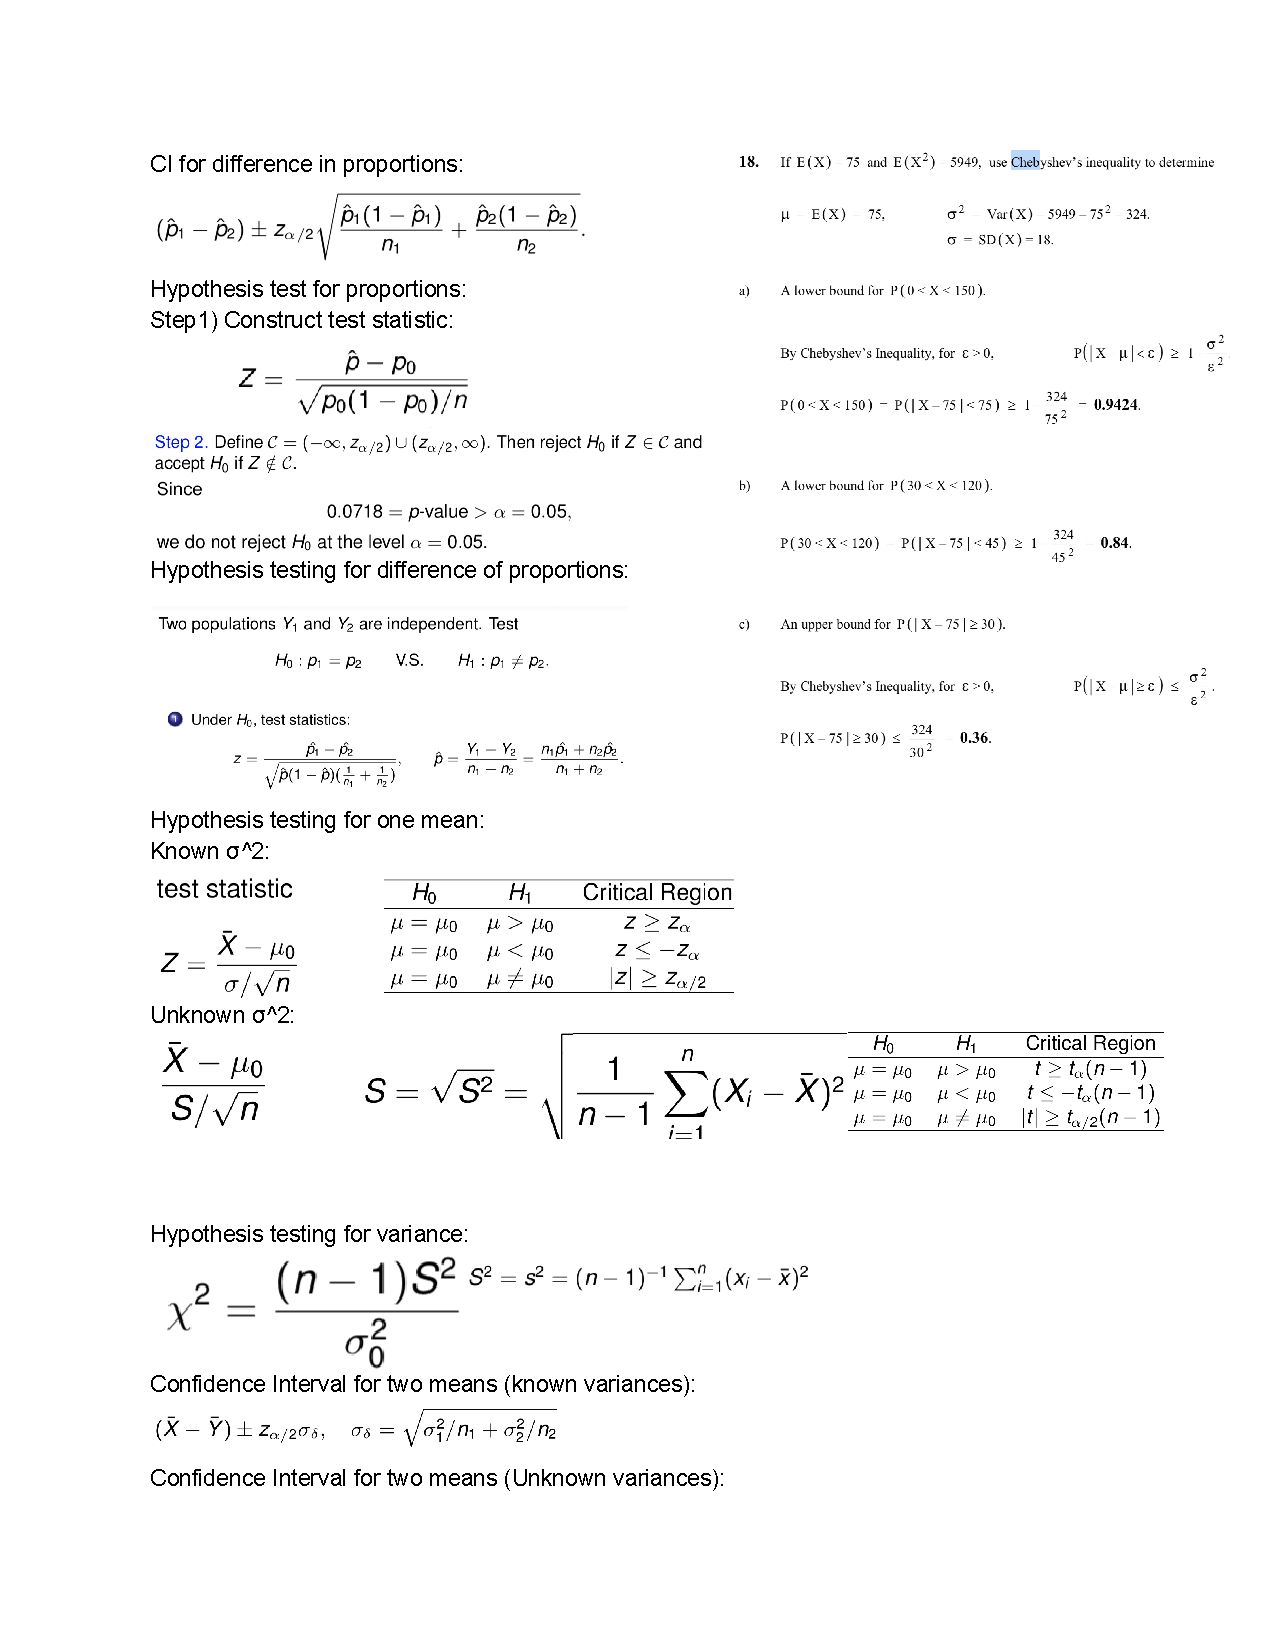
\includepdf[pages={1-},scale=1.0]{gdoc.pdf}

\end{document}